\documentclass{scrartcl} 
\usepackage[ngerman,english]{babel}
 \usepackage[T1]{fontenc}
\usepackage{lmodern}
\usepackage[applemac]{inputenc}

\usepackage{amsmath}
\usepackage{amssymb}
\usepackage{amstext}
\usepackage{amsthm}

\usepackage{fancyhdr}
\usepackage{paralist}

\usepackage{mathtools}


\usepackage{hyperref}


% PSEUDOCODE

\usepackage[ruled]{algorithm2e}


% C++ CODE

\usepackage{listings}
\usepackage{xcolor}
\definecolor{lbcolor}{rgb}{0.9,0.9,0.9}

\lstdefinestyle{customc}{
  belowcaptionskip=1\baselineskip,
  breaklines=true,
  %frame=LR,
  %xleftmargin=\parindent,
  language=C,
  showstringspaces=false,
  basicstyle=\footnotesize\ttfamily,
  keywordstyle=\bfseries\color{green!40!black},
  commentstyle=\itshape\color{purple!40!black},
  identifierstyle=\color{blue},
  stringstyle=\color{orange},
}

\lstdefinestyle{customcpp}{
	backgroundcolor=\color{lbcolor},
    	tabsize=4,
    	language=[GNU]C++,
        basicstyle=\tiny,%{\scriptsize},
        upquote=true,
        %aboveskip={1.5\baselineskip},
        columns=fixed,
        showstringspaces=false,
        extendedchars=false,
        breaklines=true,
        prebreak = \raisebox{0ex}[0ex][0ex]{\ensuremath{\hookleftarrow}},
        frame=single,
        numbers=left,
        showtabs=false,
        showspaces=false,
        showstringspaces=false,
        identifierstyle=\ttfamily,
        keywordstyle=\color[rgb]{0,0,1},
        commentstyle=\color[rgb]{0.026,0.112,0.095},
        stringstyle=\color[rgb]{0.627,0.126,0.941},
        numberstyle=\color[rgb]{0.205, 0.142, 0.73},
}

\lstset{escapechar=@,style=customcpp}


% TIKZ DIAGRAMS

\usepackage{tikz}
\usetikzlibrary{arrows}
\usetikzlibrary{positioning}

\tikzset{
    block/.style={
           rectangle,
           rounded corners,
           draw=black, very thick,
           minimum height=2em,
           inner sep=2pt,
           text centered,
           },
}

\usepackage{tikz-cd}
\tikzset{
  shift left/.style ={commutative diagrams/shift left={#1}},
  shift right/.style={commutative diagrams/shift right={#1}}
}



\DeclareMathOperator*{\esssup}{ess.sup}
\DeclareMathOperator*{\defgl}{\vcentcolon=}


%\pagestyle{fancy}
%\fancyhead[L]{Seminar \glqq Optimale Steuerung\grqq\\ Prof. Brokate, Prof. Kuttler} %Kopfzeile links
%\fancyhead[C]{} %zentrierte Kopfzeile
%\fancyhead[R]{10. Dezember 2013\\ Manuel Demmeler} %Kopfzeile rechts
\title{\vspace{-1.3cm} \textmd{\normalsize{Project description}}\\ Parallelization of the Probabilistic Roadmap Method with GPU Acceleration}
\date{}
\author{Manuel Demmeler}

%\thispagestyle{fancy}

\newcommand{\3}{ ^{3\times3} }
\newcommand{\R}{\mathbb{R}}
\newcommand{\N}{\mathbb{N}}
\newcommand{\M}{\mathbb{M}}
\newcommand{\Sym}{\mathbb{S}^3}
\newcommand{\Mpos}{\M_+^3}
\newcommand{\Orth}{\mathbb{O}^3}
\newcommand{\norm}[1]{\left\lVert#1\right\rVert}
\newcommand{\abs}[1]{\left |#1\right |}
\newcommand{\ub}{\bar{u}}
\newcommand{\yb}{\bar{y}}
\newcommand{\scprod}[2]{\langle#1 , #2 \rangle}

%\vspace{-3.4cm}


\begin{document}
\maketitle

\section{Motivation}
In trajctory optimization with obstacles, it is often necessary to provide feasible inital trajectories. 
For example in robot motion planning, where the dimensions of the underlying spaces are rather high, this can be expensive. A further problem is that because of the transformation from work into configuration space, the obstacles are often no longer given in a closed form. An efficient approximative approach is using probabilistic roadmaps (PRMs).


\section{Introduction}
\subsection{Problem Statement and the Sequential PRM Method}\label{algintro}
\newtheorem*{defi}{Definition}
\newtheorem*{alg1}{Algorithm}


The abstract problem is to find a path on a d-dimensional space, which avoids intersecting obstacles. The obstacles are  given by an indicator function
\begin{equation*}
	I: \Omega \rightarrow \{0, 1\}
\end{equation*}
on the domain \( \Omega = [ q_{min,1}, q_{max,1} ] \times ... \times  [ q_{min,d}, q_{max,d} ] \subset \R^d  \) and the goal is to find a continuous way
\begin{equation*}
	\Gamma: [0,1] \rightarrow \Omega
\end{equation*}
between a given start and endpoint, \(\Gamma(0)=q_b,\ \Gamma(1)=q_e \), 
such that
\begin{equation*}
	I(\Gamma(s))=0 \text{\ f.a.\ } s�\in [0,1].
\end{equation*}
The probabilistic roadmap (PRM) approach grows a graph \(G=(V,E)\) form \(q_s\) and \(q_e\) by randomly sampling nodes \(v\in V\subset \Omega\).  Two nodes \(v,w \in V\) are connected, if they are near enough each other and the linear connection in between is free from obstacles. The algorithm terminates, when there is a path from \(q_s\) to \(q_e\) on G.
\begin{defi}
For two points \(q_1\) and \(q_2\) we define the connection with stepsize \(h>0\) as
	\begin{equation*}
		[q_1,q_2]_h \defgl \{ q = \lambda q_1+(1-\lambda) q_2\ |\ \lambda \in [0,1], \norm{q-q_1} \in \N_0 h \}.
	\end{equation*}
	We say, \(q_1\) and \(q_2\) are connected (with stepsize \(h>0\)) on the map \(\Omega\), if
	\(I(q)=0\) for all \(q \in [q_1, q_2]_h\).
\end{defi}
\begin{alg1} (Probabilistic Roadmap in general)\\
	Input: \(q_s, q_e\in \Omega, h>0, d_0>0\)	\\
	Output: \(q_s=q_1, ... ,q_n=q_e\in \Omega\), 
		such that all \(q_i\) and \(q_{i+1}\) are connected with stepsize \(h\)
	\begin{itemize}
		\item Initialize graph \(G=(V,E)\) with \(V=\{q_s, q_e\}\), 
			if \(q_s\) and \(q_e\) are connected, \(E \leftarrow\{ q_s, q_e\}\)
		\item While there exists no path in G between \(q_s\) and \(q_e\) do
		\begin{itemize}
			\item Sample \(q\in \Omega\) from a probability density  \(p(\ \cdot\ , G)\), resample until \(I(q)=0\)
			\item \(V \leftarrow{q}\)
			\item For all nodes \(\tilde{q} \in V\) which are near enough (\( \norm{q- \tilde q} \le d_0 \)) and
				connected with \(q\) with stepsize h, 
				\(E \leftarrow \{q, \tilde{q}\}\)
		\end{itemize}
		\item Determine the shortest path \(q_1, ... , q_n\in V\) on \(G\) from \(q_s\) to \(q_e\).
	\end{itemize}
\end{alg1}


The probability density \(p(\ \cdot\ ,G)\) (depending on the actual graph) can be for example first selecting randomly a node \(q_0 \in V\) and then sampling a new point \(q\) in the neighbourhood of \(q_0\). Theory about success probabilities and convergence results can be found in \cite{prmlec}, \cite{prm1} or \cite{prm2}.


\subsection{Application to Robotics}


\begin{figure}
    \centering
    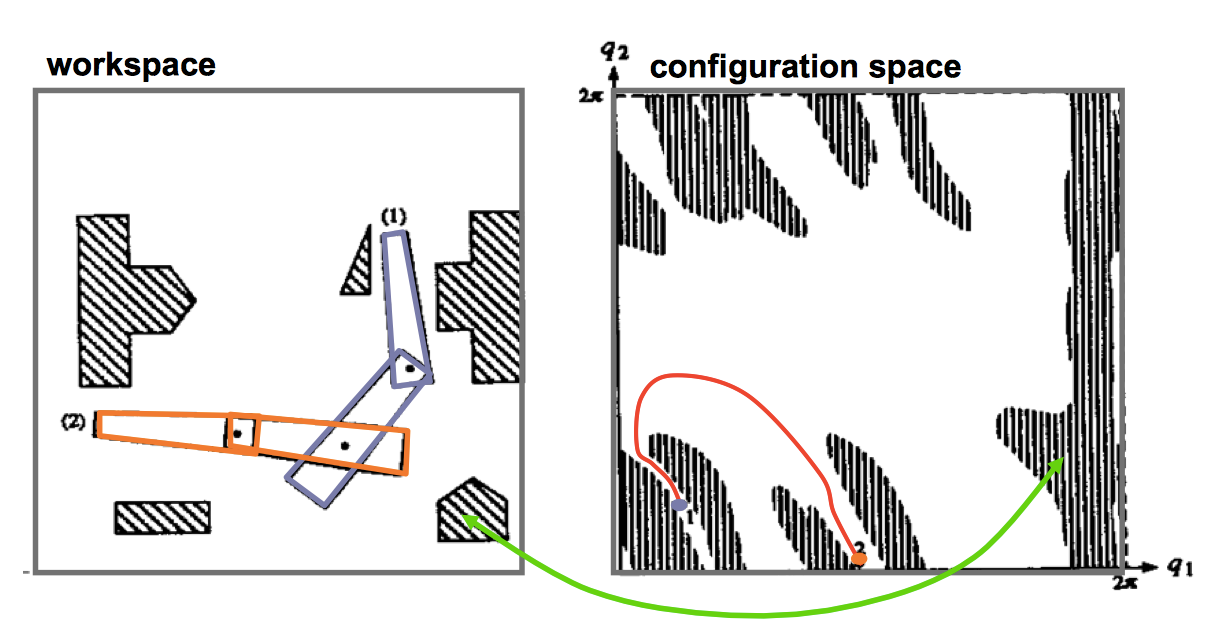
\includegraphics[width=0.8\textwidth]{configspacetrafo.png}
    \caption{Example for an indicator function in robotics from \cite{prmlec}. 
    		The real obstacles on the left are transformed 
		into occupied areas of the configuration space on the right.}
    \label{fig:awesome_image}
\end{figure}

In the project, the PRM algorithm is used to find trajectories for a robot arm, which avoid self collisions and collisions with obstacles in the environment.
Such trajectories can be expressed as functions describing the joint variables changing over time, that means curves in the configuration space with dimension equal to the number of degrees of freedom of the robot.
With this association, the trajectory finding problem becomes a path finding problem in the configuration space exactly of the form stated in the previous chapter.
The real obstacles transform into obstacles in the configuration space, given by the indicator function, that returns for a given set of joints, if the configuration is feasible or a collision occurs.



\subsection{Project Overview}

Like in the stated robotics example, in many cases the most costly operation of the PRM algorithm are the many evaluations of the indicator function \(I(q)\), 
which however can be done independently for every new \(q\).
Therefore $I(q)$ is implemented in a vectorized way as a function \((q_1, ... , q_P) \mapsto (I(q_1),...,I(q_P))\) by a CUDA kernel, where every thread computes one evaluation.
In the robotics case, this means, the direct kinematic and collision calculation are made on the GPU parallely for different joint angle configurations.
Although this will the only major application in the project, the PRM solver and the configuration space are implemented seperated from each other and connected by an interface to be free to simply add other applications. As an example and for testing, additionally a simple 2D configuration space is provided, 
whose indicator function is read from a black-and-white image.

\ \\ 
\begin{tikzpicture}[auto]%node distance=0.5cm and 1.8cm]
	\node[block] (prm) {
		\begin{tabular}{c}
		\textbf{PRMSolver}\\
		generate nodes\\
		store graph
		\end{tabular}
	};
	\node [block, right=of prm] (config) {
		\begin{tabular}{c}
		\textbf{Configpace}\\
		indicator fct. \\
		interface
		\end{tabular}
	};
	\node [block, right=of config] (robo) {
		\begin{tabular}{c}
		\textbf{RobotConfigspace}\\
		robot kinematics\\
		collision detection
		\end{tabular}
	};
	\node [block, right=of robo] (gpu) {\textbf{GPU}};
	
	\path[-stealth,thick, shift left=1.0ex]	(prm) edge (config) ;
	\path[-stealth,thick, shift left=1.0ex]	(config) edge  (prm) ;
	\path[-stealth,thick, shift left=1.0ex]	(config) edge (robo);
	\path[-stealth,thick, shift left=1.0ex]	(robo) edge  (config);
	\path[-,thick]					(robo) edge (gpu);
\end{tikzpicture}
\ \\ 

Then in a first level of parallelization, this function can be applied to the \(q_i \in [q, \tilde q]_h \) to check, if \(q\) and \(\tilde q\) are connected.



Furthermore, a second level of parallelization could be achieved by sampling and connecting several new points \(\tilde q_i\) parallely. This is expected to be more difficult, because all new nodes have to be connected to the old graph and to each other. Therefore it has to be evaluated, if a parallel implementation stays efficient here.


If there remains time, a next idea could be to execute the algorithm on different discretization levels \(h\). This means for example to compute a way \(q_1^0, ..., q_n^0\) which is connected with a coarse stepsize \(h_0\), then to decrease the stepsize to \(0<h_1<h_0\) and take the path nodes \(q_i^0\) as starting nodes for the next execution of the algorithm, which gives then an \(h_1\)-connected way \(q_1^1, ... , q_n^1\), etc.




\section{Structure of the PRM Solver}

here overview over the components of the programm components: 

PRMSolver 1 <-> Configspace object 1 <-> GPU 1

.

.

.

PRMSolver n <-> Configspace object 2 <-> GPU 1


- description of the different versions:

- definitions as pseudocode

version 1: 

	- each process generates own nodes -> exchange them, synchronous gpu kernel

version 2: 

	- every process generates all nodes (same by exchange of random seed)

	- indicator function splitted over processes, synchronous

version 3: 

	- same as version 2 with some pipeline optimizations

version 4:

	- same as version 3 with asynchronous gpu

version 5:

	- each process has 2 workers which are generating their nodes an are using 1 gpu

	- one worker uses the kernel time  of the other to do its work

	- should give use the gpu computation time efficiently


\section{Implementation of an Indicator Function for Robot Arms}

In the project, the probabilistic roadmap algorithm is applied  to create collisionfree trajectories of a robot arm.
For a robot with given joint angles \(q_i\) one can calculate straightforwardly all positions and orientations  of the single parts of the robot.
For this, coordinate frames according to the Denavit-Hartenberg convention are used.
The coordinate frames of the single parts are described by transformation matrices 
$T_i \in R^{4x4}$, which transform points of the body frame into the world frame. They depend on the state $q=(q_1,...,q_d)$ of the robot and on the geometry of the joint angles given by the Denavit-Hartenberg parameters of the robot. 

The geometry of the robot parts is defined by a set of convex polytopes, each of them belonging to one of the robots coordinate frame. Applying the corresponding $T_i$, its vertices can be transformed into the world frame. 
Environment obstacles are also defined by convex polytopes, in the world frame.

Now the movement of the robot can be described by a curve $q(t)$ in the state space. It is collisionfree, if at no time, any two polytopes of the robot intersect with each other or with the environment after transformed into the world frame.
To apply the probabilistic roadmap algorithm, we express this by the indicator function

\begin{equation*}
	I(q)=
	\begin{cases}
		0,	& \text{ for no collision for all given pairs of polytopes in wold frame } \\
		1,	& \text{ if at least one collision occurs }
	\end{cases}
\end{equation*}

It has to be noted that the trajectories \(q(t)\) the PRM algorithm generates are piecewise linear and therefore not differentiable. Hence, they have to be smoothed before the use on a robot. This is not part of the project. The task is only to generate feasible trajectories to be passed to an optimizer.


The indicator function is implemented in a vectorized way as an CUDA kernel, which means that, given set of states $q^1,..,q^M$, the indicator function is evaluated for each state by one CUDA thread. Therefore, the kinematics and collision algorithm have been implemented as device code for the use in the kernel.

\subsection{Direct Kinematics}\label{dk}

The Denavit-Hartenberg (DH) convention is a method to describe the geometry of an robots joints, 
that is, how the transformations between the robots coordinate frames look like in dependancy of its joint values $q_1,...,q_d$.
For this it is assumed that each joint is either rotational, that means an rotation around a fixed axis, 
or prismatic, a translation along an axis.
The robot consists of $d+1$ bodies each of which has an body fixed coordinate frame $B_i$, which is described by the transformation matrix $T_i$ into the world frame.
For an robot with DH parameters $a_{i-1}, \alpha_{i-1}, d_i \in \R$, $i=1,...,d$, 
the relative transformations $T_{i-1,i}=T_{i-1}^{-1} T_{i}$ between two bodies now is defined as
\begin{equation}
	T_{i-1,i} = R_z(\theta_i) T_z(d_i) R_x(\alpha_{i-1}) R_x(a_{i-1})
\end{equation}
where $R_x, R_z$ are rotations and $T_x, T_z$ translations around the $x$ and $z$ axes.
By an proper choice of the body frames, every robot with rotational or prismatic joint can be described by DH parameters.
For the exact calculations, see \cite{robodyn}.


\subsection{2D and 3D Geometry Library}

For the CUDA implementation of the kinematics and later the collision algorithm, a geometry library was written, based on the CUDA datatypes float2 for 2D vectors and float4 for 3D vectors.
To guarantee aligned access on the GPU, float4 is used instead of float3. Furthermore, as the geometric calculations made here are numerically not very critical, the usage of double precision has turned out to be not necessary.
The library contains hybrid host and device inline functions for common vector operations such as
\begin{lstlisting}
__host__ __device__ inline float4& operator += (float4& u, const float4& v);
__host__ __device__ inline float4& operator *=  (float4& u, const float f);
__host__ __device__ inline float4& add(const float4& u, const float4& v, float4& w);
\end{lstlisting}
Operators like $+$ or $*$ are not overloaded to prevent unnecessary temporary variables.

Transformation matrices are implemented float4 arrays with inline functions for common matrix operations. Again operators with temporaries avoided.
\begin{lstlisting}
class trafo4{
  public:
    float4 col[4];
    __host__ __device__ trafo4(){}
    __host__ __device__ trafo4(float a, float alpha, float q, float d);
    __host__ __device__ inline float4& apply(float4& u) const;
    __host__ __device__ inline float4& apply(const float4& u, float4& Tu) const;
    .
    .
    .
}
\end{lstlisting}

\subsection{Polytopes}

To calculate the intersection between two polytopes, the Chung-Wang algorithm only needs their vertices 
and the data which vertices are connected by an edge. 
For this the adjacency matrix of the edge graph is stored compactly in the crs format.
\begin{lstlisting}
struct polytope4{
    float4* vertices;	//length n
    int n;
    //!edges in crs format
    int* dsp;	//length n
    int* cnt;	//length n
    int* dest;	//length m
    int m;
};
\end{lstlisting}
It means, that for $i=0,...,n-1$ the vertices $dest[dsp[i]],...,dest[dsp[i]+cnt[i]-1]$ are the ones connected with vertex $i$ by an edge.


- whole list of polytopes stored compactly in polytope4data on gpu

- maybe describe interface polytope <-> polytope4data <-> polytope4






\subsection{Chung-Wang Collision Algorithm}

To check if two polytopes collide an algorithm by Chung and Wang is used here. It uses the separating vector theorem and tries to find a seperating vector by iterative search. Furthermore, a subalgorithm determines in each iteration from the candidate history, if it is still theoretically possible to find a seperating vector. If not, it is returned a collision. If on the other side a seperating vector is found, the algorithm can return no collision.
For detailed informations see \cite{chung} and \cite{ericson}, pp. 410-412.
The method is implemented as device code for the use on GPU kernels.
\begin{lstlisting}
__host__ __device__ int seperating_vector_algorithm(const polytope4& P, const polytope4& Q, 
													const trafo4& tp, const trafo4& tq);
\end{lstlisting}
In our application, the polytopes are mostly parts of the robot, which are given in a body frame and have to be transformed into world frame according to section \ref{dk} first.
However, from the structure of the Chung-Wang algorithm drops out that mostly only a small part of the polytopes vertices are needed for the computations. Therefore it would be rather time wasting to transform all vertices before passing to the algorithm. To avoid this, all polytopes are passed in their body frames together with their transformations and the algorithm transforms vertices at the time they occur in calculations.





\subsection{Robot Kernel}

The robot configuration space is implemented in the form
\begin{lstlisting}
template<int ndof>
class RobotConfigspace : public Configspace<ndof>
{
public:
  RobotConfigspace(const Robot<ndof>* robot_,
                   const polytope *polys_,
                   const int* sys_,
                   const int N_,
                   const int *from_, const int *to_,
                   const int M_,
                   const float* mins_, const float* maxs_, const float dq_,
                   const int nbuf_);
  int init(const int ressource_rank=0, const int ressource_size=1);
  int indicator2(const float* qs, const float* qe, int *res, const int N, const int offset);
  .
  .
  .
private:
  const Robot<ndof>* robot; //host
  Robot<ndof>* robotdev;    //GPU
  collision4::polytope4data* polydata;            //data on host
  collision4::polytope4data* polydatadev;         //pointer to GPU obj
  .
  .
  .
}
\end{lstlisting}
\begin{lstlisting}
__global__ void kernel_indicator2(const Robot<ndof>* robot,
                                  const collision4::polytope4data* polydata,
                                  const float* qs, int offsets,
                                  const float* qe, int offsete,
                                  int* res,
                                  const int* testpos, const int* testnum,
                                  int N, int numthreads);
\end{lstlisting}
where the constant geometry and robot data is passed once at the beginning and copied to the GPU by an init function.
The indicator function gets as input a list of border points $q_{start}^j, q_{end}^j, j=0,...,N$ and checks now for each pair, if on the line in between the indicator function is always 0.
\begin{equation}
	res[j]=\begin{cases}
		0	&\text{if $I(q)=0$ f.a. $q \in \left[qs[j], qe[j]\right]_{\Delta q}$} \\
		1	&else
	\end{cases}
\end{equation}
The border points are stored in structures of arrays.
\begin{equation}
\begin{aligned}
	q_{start}^j &= \left(qs[j],qs[j+\text{offset}],...,qs[j+(d-1)*\text{offset}]\right)^T\\
	q_{end}^j &= \left(qe[j],qe[j+\text{offset}],...,qe[j+(d-1)*\text{offset}]\right)^T
\end{aligned}
\end{equation}

As the PRMSolver only needs to know, which node points can be connected by a line, and not, which points on the line exactly are free, this version delivers exactly the minimal necessary information. Furthermore it saves CPU and communication time, because the intermediate points on the lines can be directly computed by the GPU threads and do not need to be exchanged.

Algorithms 1 and 2 two show in pseudo code, how the work is split between host and device.


\begin{algorithm}
	\KwData{qs, qe, N, offset}
	\KwResult{res}
	compute distances $d_j = \abs{q_{end}^j - q_{start}^j}$ \;
	testnum[j] = $d_j/{\Delta q}$: number of threads for each line \;
	testpos[j] = thread displacements \;
	reset res \;
	call kernel \;
	\caption{Host indicator function}
\end{algorithm}

\begin{algorithm}
	\KwData{arrays qs, qe, testpos, testnum and threadindex}
	\KwResult{res}
	compute associated edge number $j$, defined by $testpos[j] \leq threadindex \le testpos[j]+testnum[j]$ \;
	$c = (threadindex - testpos[j]) / (testnum[k]-1) $ \;
	$q=c q_{start}^j + (1-c) q_{end}^j $ \;
	calculate robot kinematics $T_0(q), ..., T_d(q) $\;
	$res_{tmp} = 0; $ \;
	\For{all registered pairs pairs of polytopes $P, Q$}{
		$res_{tmp}=seperating\_vector\_algorithm(P, T_{i_P}, Q, T_{i_Q})$ \;
		\If{$res_{tmp} \neq 0$}{
			$res[j]=res_{tmp}$ \;
			break \;
		}
	}
	\caption{Robot kernel: code for one thread}
\end{algorithm}

In order to overlap computation time of GPU and CPU, an asynchronous version of the indicator function was written. Here the function is split in everything until the kernel launch and a wait function, which waits until the kernel finishes and recieves the result data. 

\begin{lstlisting}
int indicator2_async(const float* qs, const float* qe, int *res, 
					 const int N, const int offset, int &request);
int indicator2_async_wait(int request);
\end{lstlisting}

The implementation also allows overlapping of multiple requests, for example two calls of the launch function and after this the two corrsponding waiting calls. 
With this it is possible to use the full computation time of the GPU.


\bibliographystyle{alpha}
\begin{thebibliography}{999}
	\bibitem{prmlec} D. Burschka, Lecture Robot Motion Planning, source: http://robvis01.informatik.tu-muenchen.de/courses/wegtraj/index.html
	\bibitem{prm1} H. Choset, K. Lynch, S. Hutchinson, G. Kantor, W. Burgard, L. Kavraki and S. Thrun, Principles of Robot Motion: Theory, Algorithms, and Implementation, MIT Press, 2005
	\bibitem{prm2} S. M. LaValle, Planning Algorithms, Cambridge University Press, 2006
	\bibitem{robodyn} T. Buschmann, Skript zur Vorlesung: Roboterdynamik SS14, Lehrstuhl f�r Angewandte Mechanik, TU M�nchen, 2014
	\bibitem{chung} K. Chung, Wenping Wang, Quick Collision Detection of Polytopes in Virtual Environments, Proceedings of the ACM Symposium on Virtual Reality Software and Technology (VRST 96), Mark Green (ed.), 1996
	\bibitem{ericson} C. Ericson, Real-Time Collision Detection, Elsevier, 2005
\end{thebibliography}

\end{document}


















